\section{Sinusoidal $f(t)$ with Shifted Time Box Kernel}
In this analysis, we investigate the convolution of a sinusoidal input signal $f(t) = A\sin(\omega t + \phi)$ with a rectangular kernel that is shifted by $\tau_0$. The shifted rectangular kernel is defined as:

$$
h(t)= \begin{cases}
1, & \text{for } \tau_0-T < t < \tau_0+T \\
0, & \text{otherwise}
\end{cases}
$$

Our goal is to derive the convolution expression $y(t)=(f * h)(t)$ analytically and analyze the system's behavior.

\subsection{Analytical Derivation}

The convolution of $f(t)$ and $h(t)$ is defined as:

$$
y(t) = (f * h)(t) = \int_{-\infty}^{\infty} f(\tau)h(t-\tau)d\tau
$$

Substituting our functions:

$$
y(t) = \int_{-\infty}^{\infty} A\sin(\omega \tau + \phi) \cdot h(t-\tau)d\tau
$$

Since the kernel $h(t-\tau)$ is non-zero only when $\tau_0-T < t-\tau < \tau_0+T$, we can rewrite this as:

$$
t-\tau_0-T < \tau < t-\tau_0+T
$$

Therefore, the limits of integration become:

$$
y(t) = \int_{t-\tau_0-T}^{t-\tau_0+T} A\sin(\omega \tau + \phi)d\tau
$$

Evaluating this integral:

\begin{align*}
y(t) &= A\int_{t-\tau_0-T}^{t-\tau_0+T} \sin(\omega \tau + \phi)d\tau \\
&= -\frac{A}{\omega}[\cos(\omega \tau + \phi)]_{t-\tau_0-T}^{t-\tau_0+T} \\
&= -\frac{A}{\omega}[\cos(\omega(t-\tau_0+T) + \phi) - \cos(\omega(t-\tau_0-T) + \phi)]
\end{align*}

Using the trigonometric identity $\cos(\alpha) - \cos(\beta) = -2\sin\left(\frac{\alpha+\beta}{2}\right)\sin\left(\frac{\alpha-\beta}{2}\right)$:

\begin{multline*}
    y(t) = -\frac{A}{\omega}\left[-2\sin\left(\frac{\omega(t-\tau_0+T) + \phi + \omega(t-\tau_0-T) + \phi}{2}\right)\right] \\ \left[\sin\left(\frac{\omega(t-\tau_0+T) + \phi - (\omega(t-\tau_0-T) + \phi)}{2}\right)\right]
\end{multline*}
\begin{align*}
y(t) &= -\frac{A}{\omega}\left[-2\sin(\omega(t-\tau_0) + \phi)\sin(\omega T)\right] \\
    \implies y(t) &= \frac{2A\sin(\omega T)}{\omega}\sin(\omega(t-\tau_0) + \phi)
\end{align*}

We can see that this result is similar to the case where shift does not happen. The main difference which is seen that the convolution output is shifted by an exact amounnt $\tau_0$.

\subsection{Analysis of the Result}

The convolution result can be expressed as:

$$
y(t) = \frac{2A\sin(\omega T)}{\omega}\sin(\omega(t-\tau_0) + \phi)
$$

This shows that:

\begin{enumerate}
\item The output is still a sinusoidal function with the same frequency $\omega$ as the input.

\item The amplitude is scaled by a factor of $\frac{2\sin(\omega T)}{\omega}$, which depends on both the frequency of the input signal and the half-width $T$ of the rectangular kernel.

\item The phase of the output signal is shifted by $\tau_0$, which corresponds to the shift in the rectangular kernel.

\end{enumerate}

\begin{figure}[!ht]
    \begin{center}
        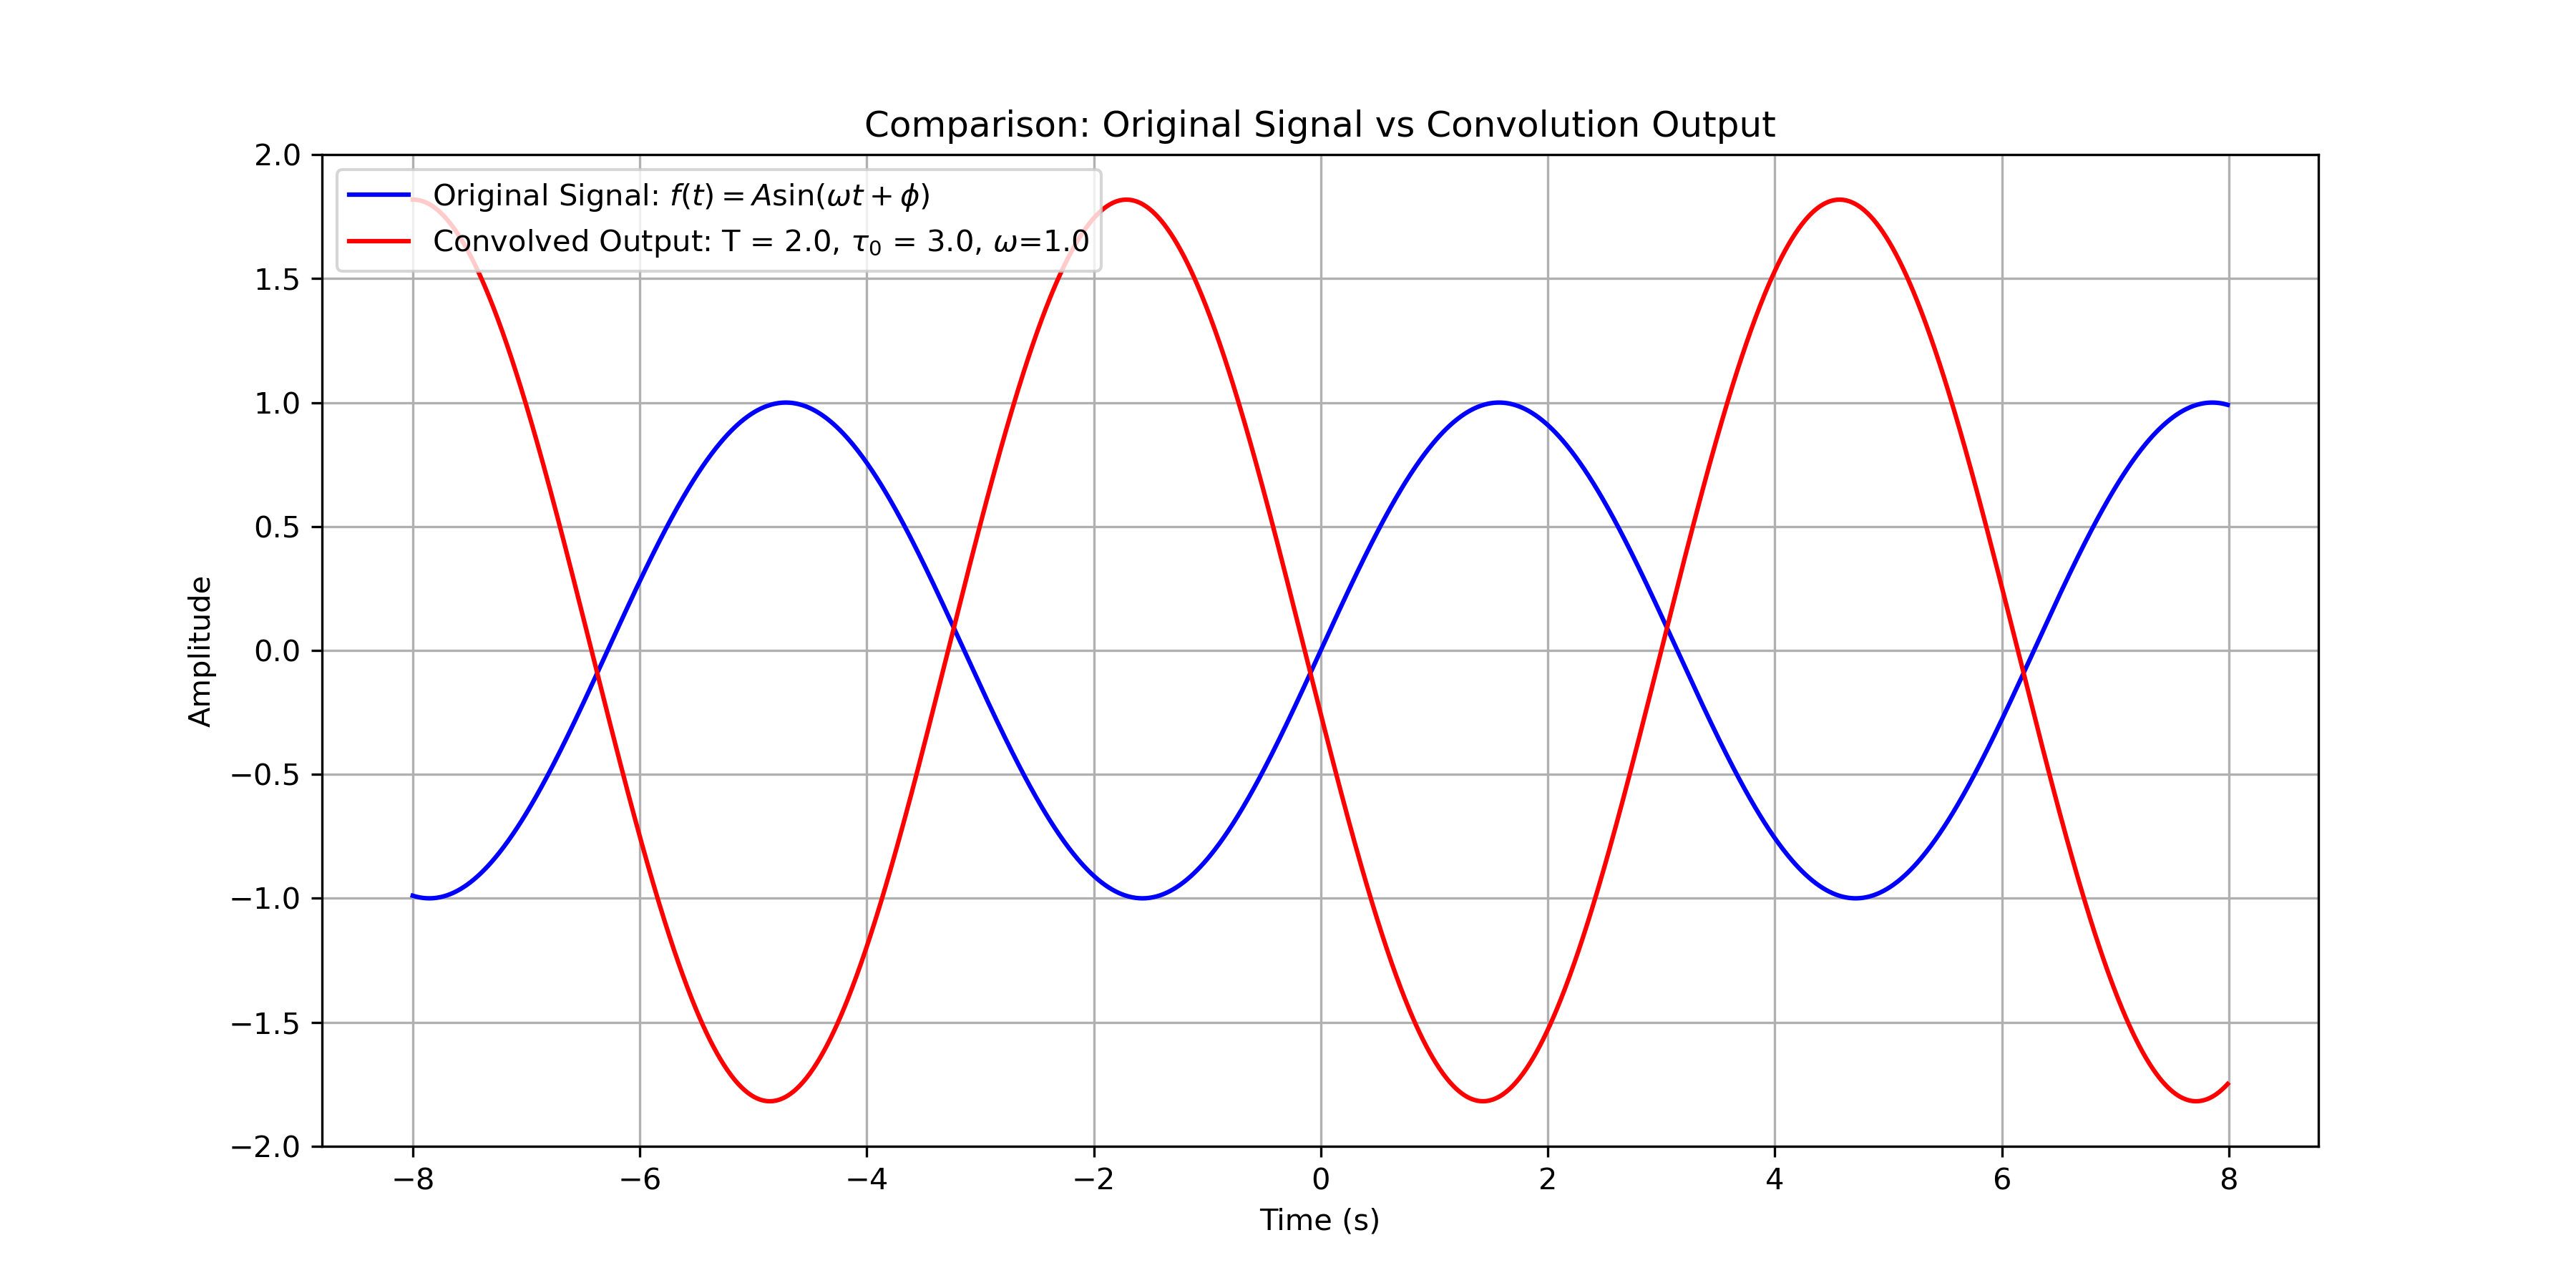
\includegraphics[width=0.95\textwidth]{codes/codes_sin_3_and_smoothening/figs/original_vs_convolved.png}
    \end{center}
    \caption{Original Signal vs Convolved Signal plot}
\end{figure}
\FloatBarrier

\subsection{Effect of Kernel Shift $\tau_0$}

The shift $\tau_0$ in the kernel results in a time delay in the output signal. This is evident from the term $\sin(\omega(t-\tau_0) + \phi)$ in our result. This demonstrates an important property of convolution: a shift in one of the functions results in an equivalent shift in the convolution result.

In the context of time-delayed systems, this shows that the system introduces a delay of $\tau_0$ in the response. This could represent physical phenomena like signal propagation delays in communication systems or processing delays in control systems.

\begin{figure}[!ht]
    \begin{center}
        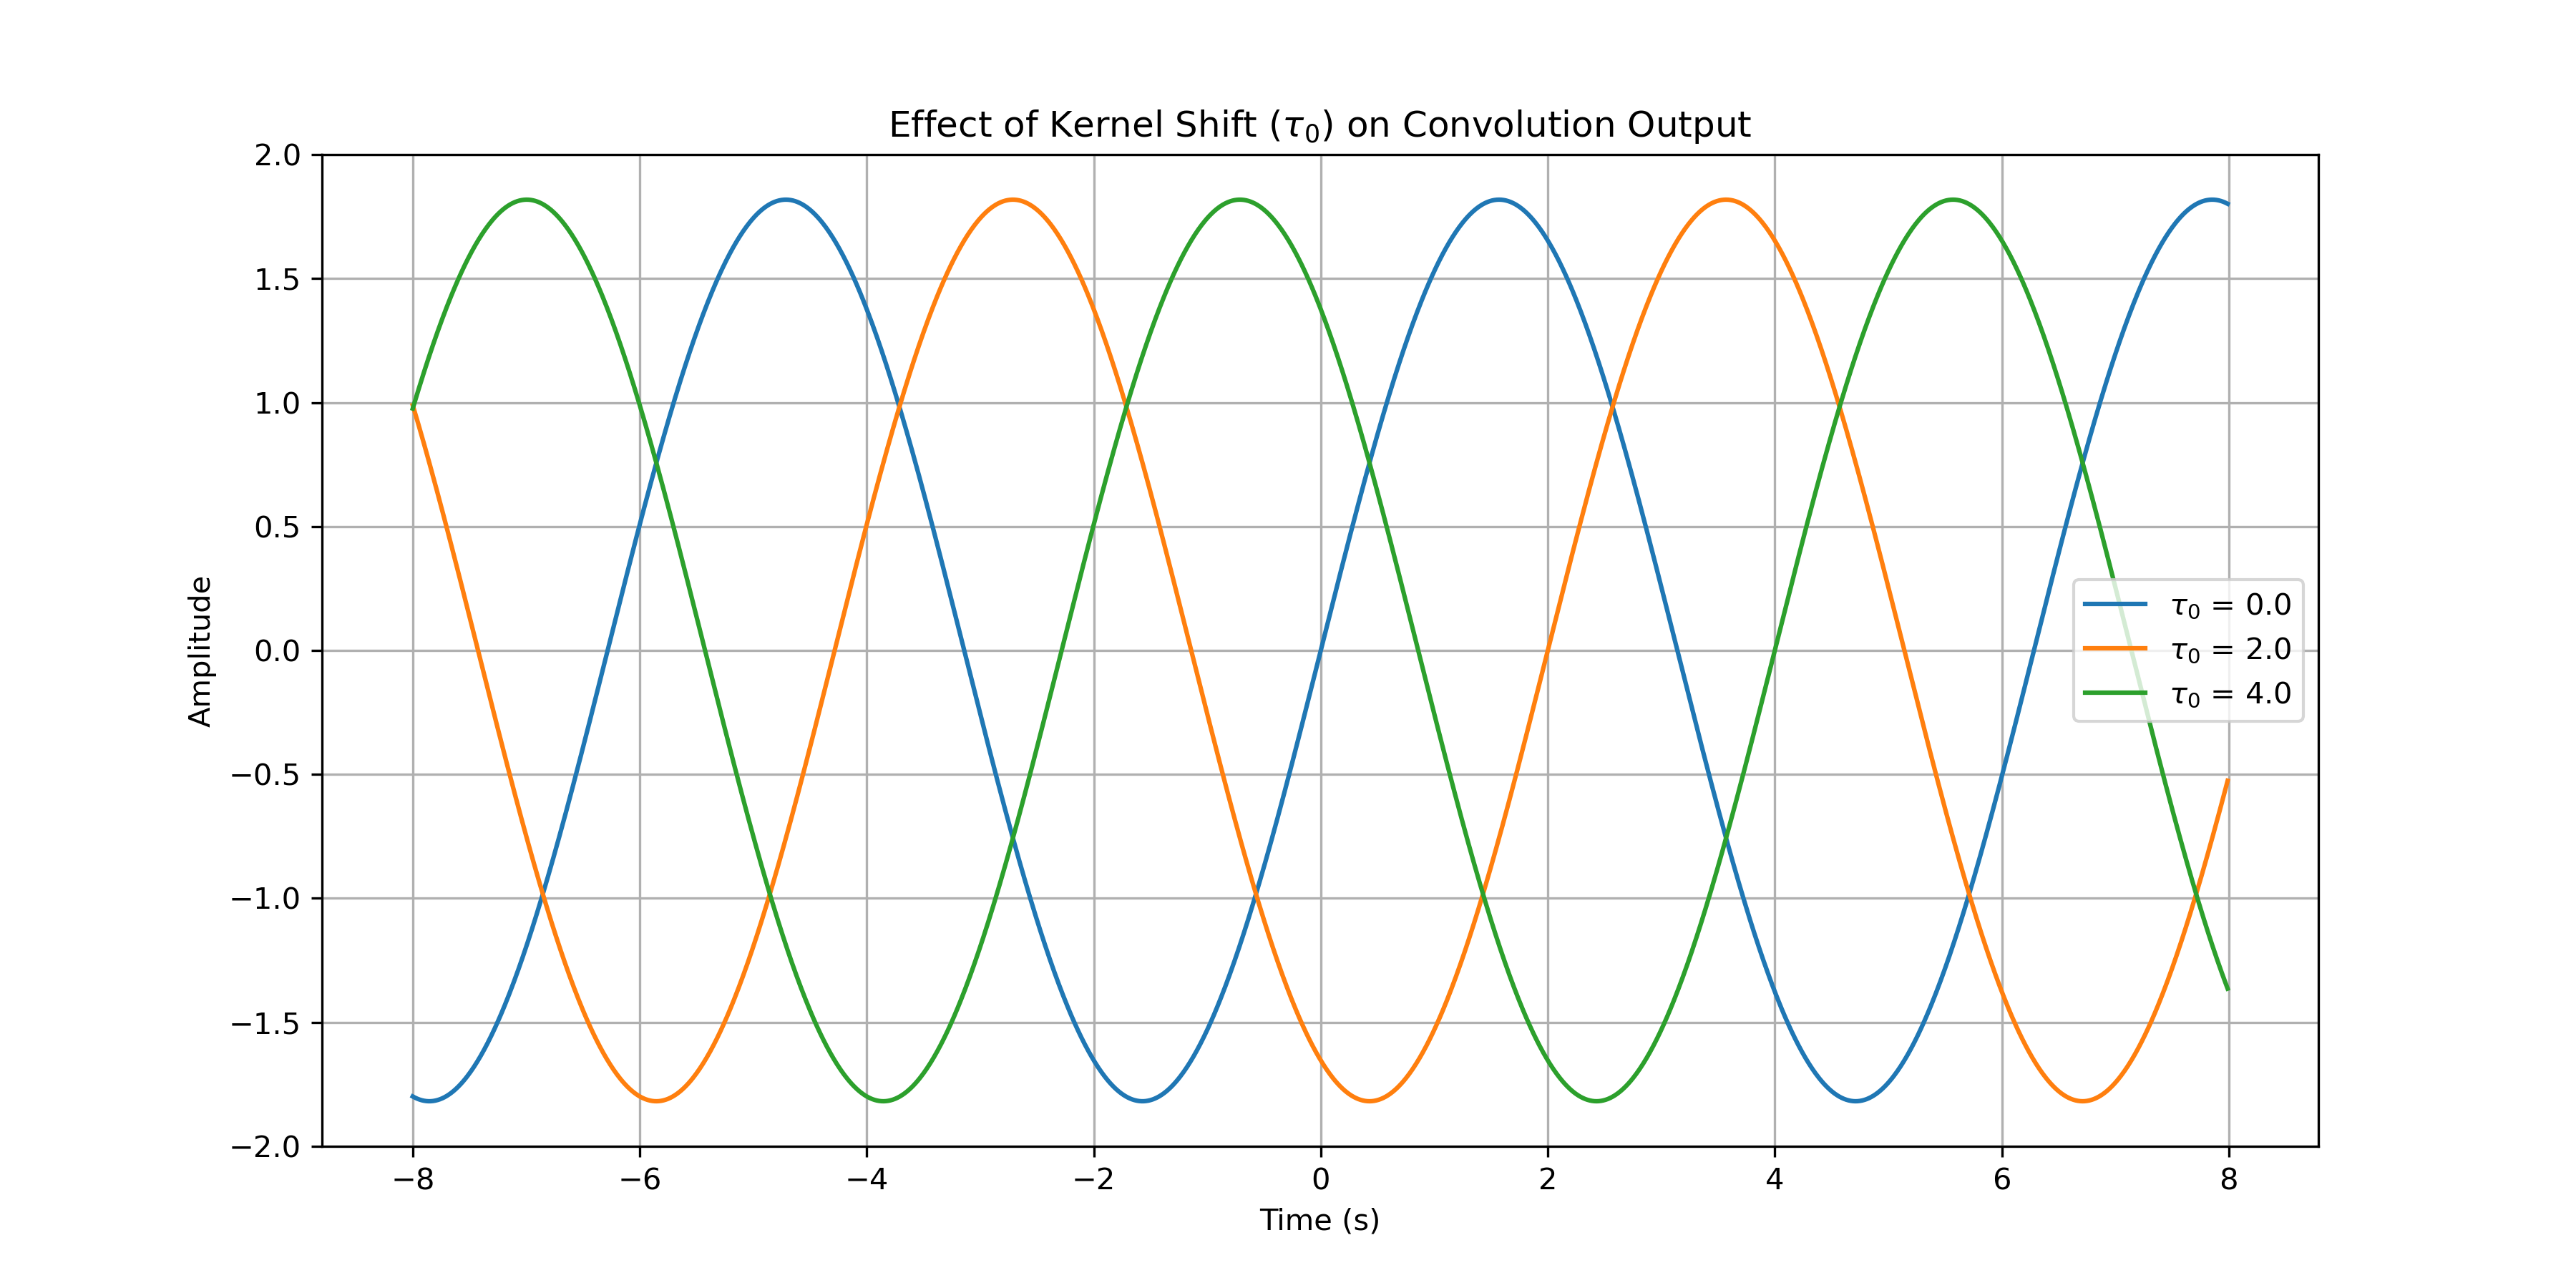
\includegraphics[width=0.95\textwidth]{codes/codes_sin_3_and_smoothening/figs/varying_tau_effect.png}
    \end{center}
    \caption{Effect of $\tau_0$ on the convoluted signal}
\end{figure}
\FloatBarrier

\subsection{Special Cases}

\begin{enumerate}
\item When $\omega T = n\pi$ (where $n$ is a non-zero integer), $\sin(\omega T) = 0$, making the output zero. This represents frequencies that are completely filtered out by the system.

\begin{figure}[!ht]
    \begin{center}
        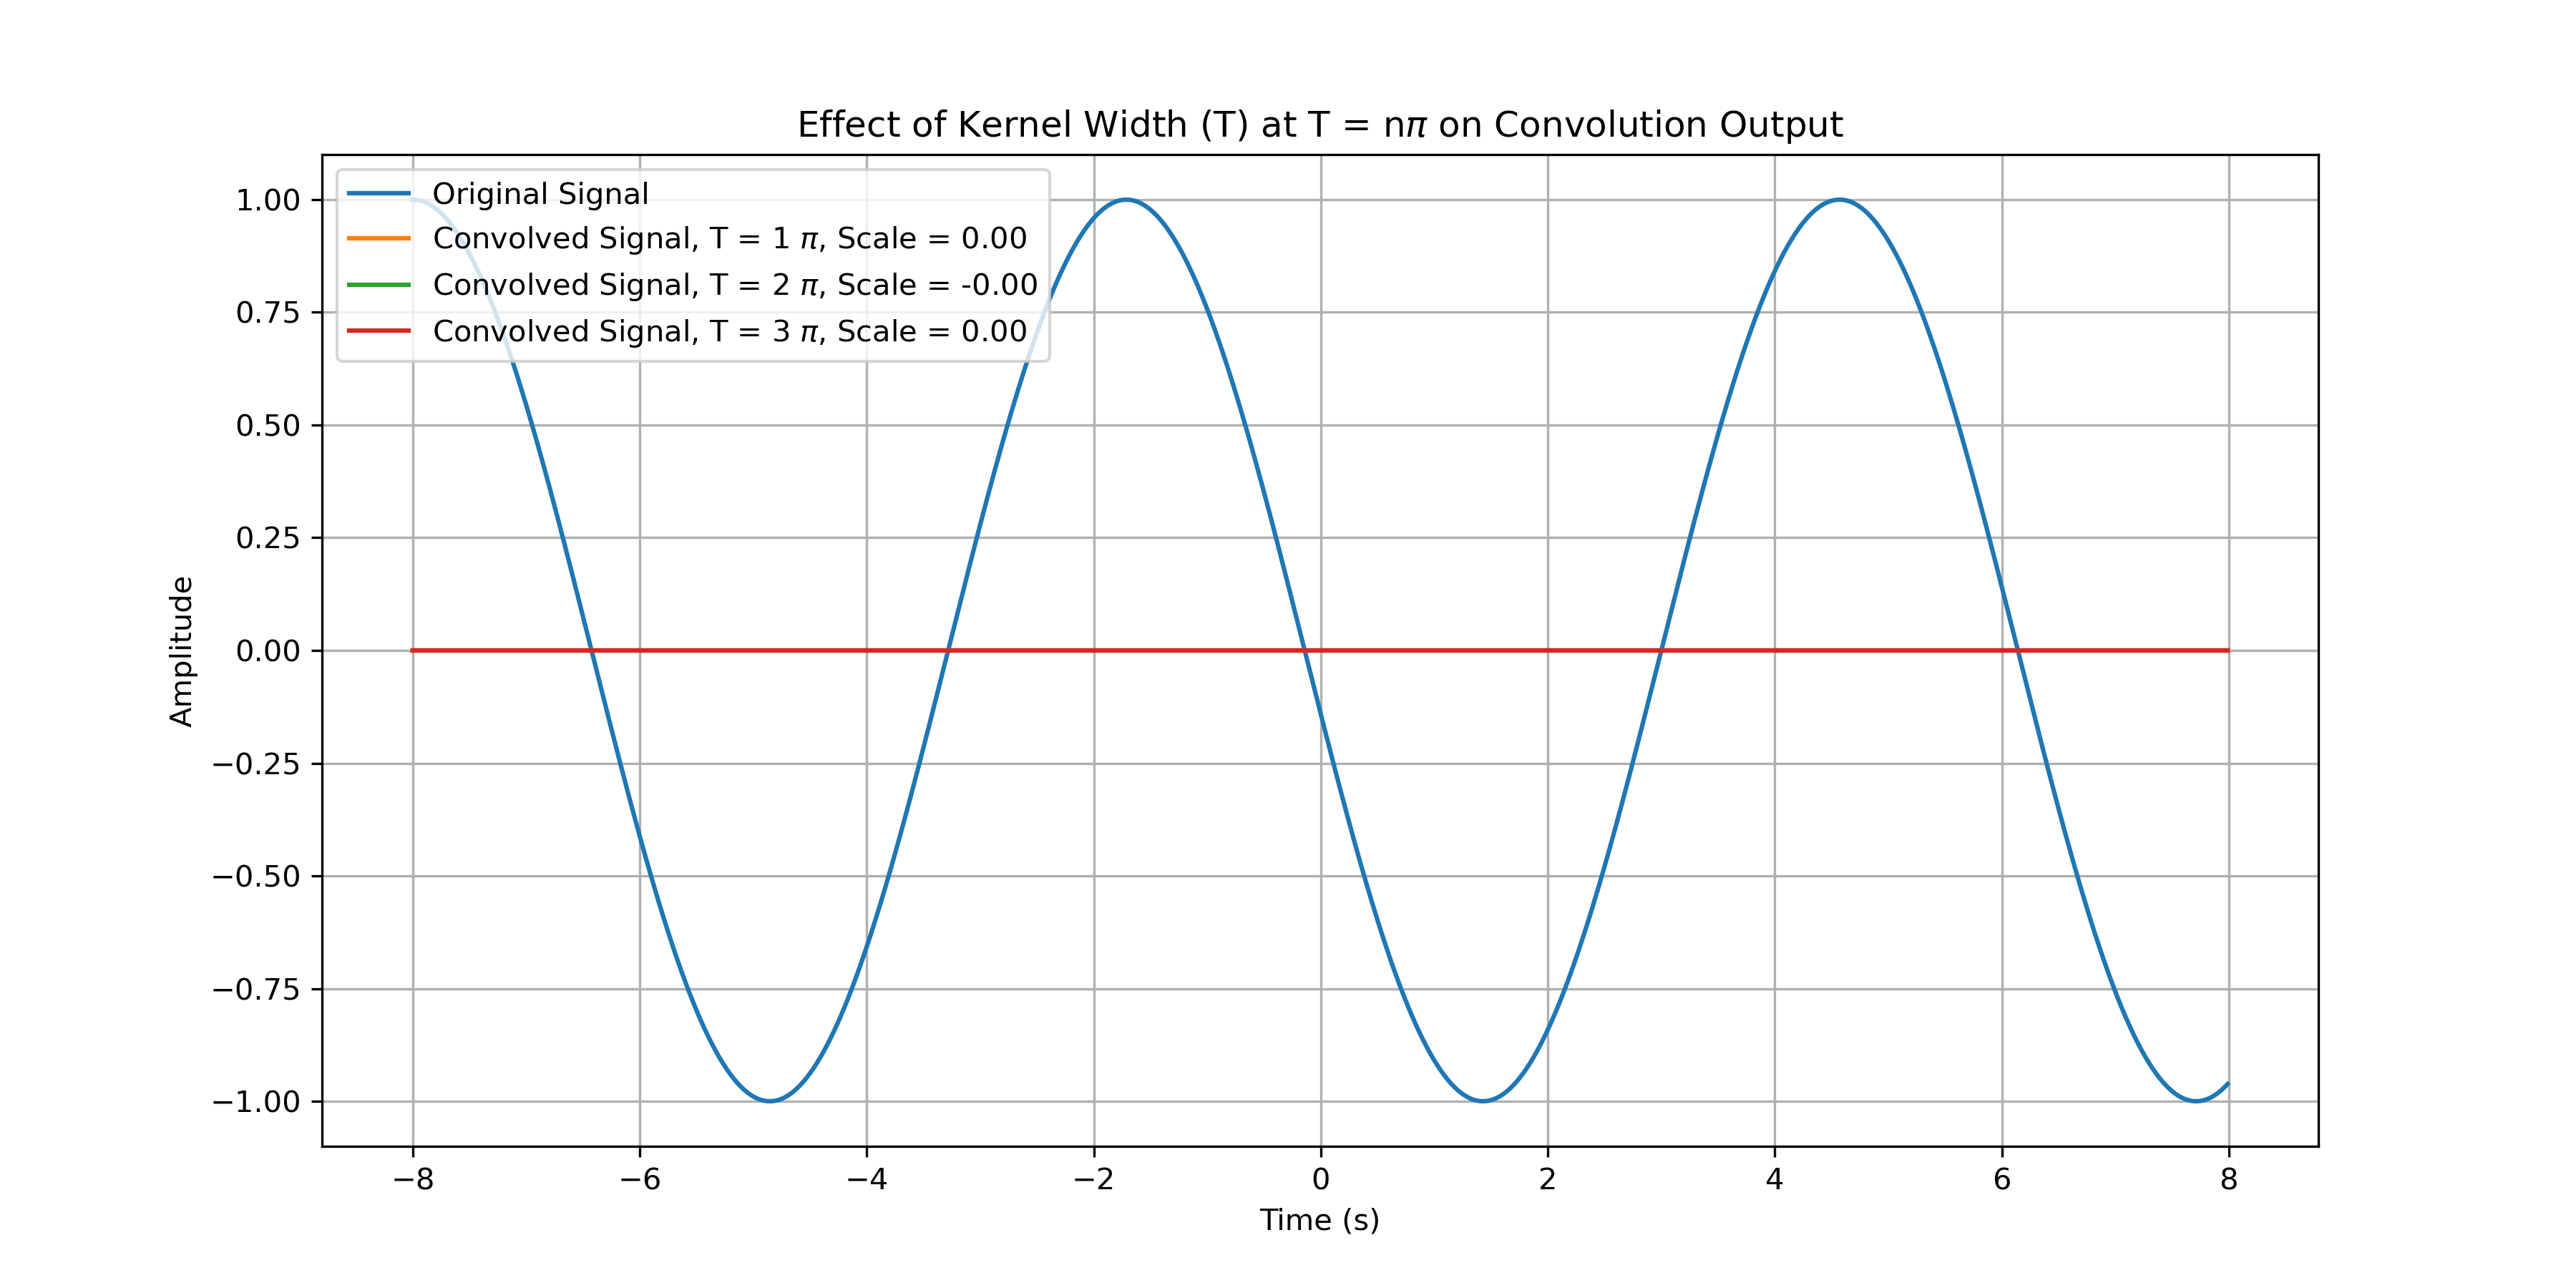
\includegraphics[width=1\textwidth]{codes/codes_sin_3_and_smoothening/figs/varying_T_pi_effect.png}
    \end{center}
\end{figure}
\FloatBarrier

\item When $T$ approaches zero, the kernel approaches a unit impulse function, and the output approaches zero for all $t$.

\item When $T$ is very large, the term $\frac{\sin(\omega T)}{\omega}$ oscillates, but its amplitude decreases as $\frac{1}{\omega}$, acting as a low-pass filter.
\end{enumerate}

\subsection{Amplitude ratio Analysis}
Amplitude ratio is given by:
\begin{align}
    \frac{A_{out}}{A_{in}} = \frac{2\sin{\omega T}}{\omega} = 2T sinc(\omega T)
\end{align}

As you can observe, it is a typical $sinc$ function which dies down as $\omega$ increases. This makes it an interesting way to filter out high frequencies, effectively making it a working but crude low-pass filter.

\begin{figure}[!ht]
    \begin{center}
        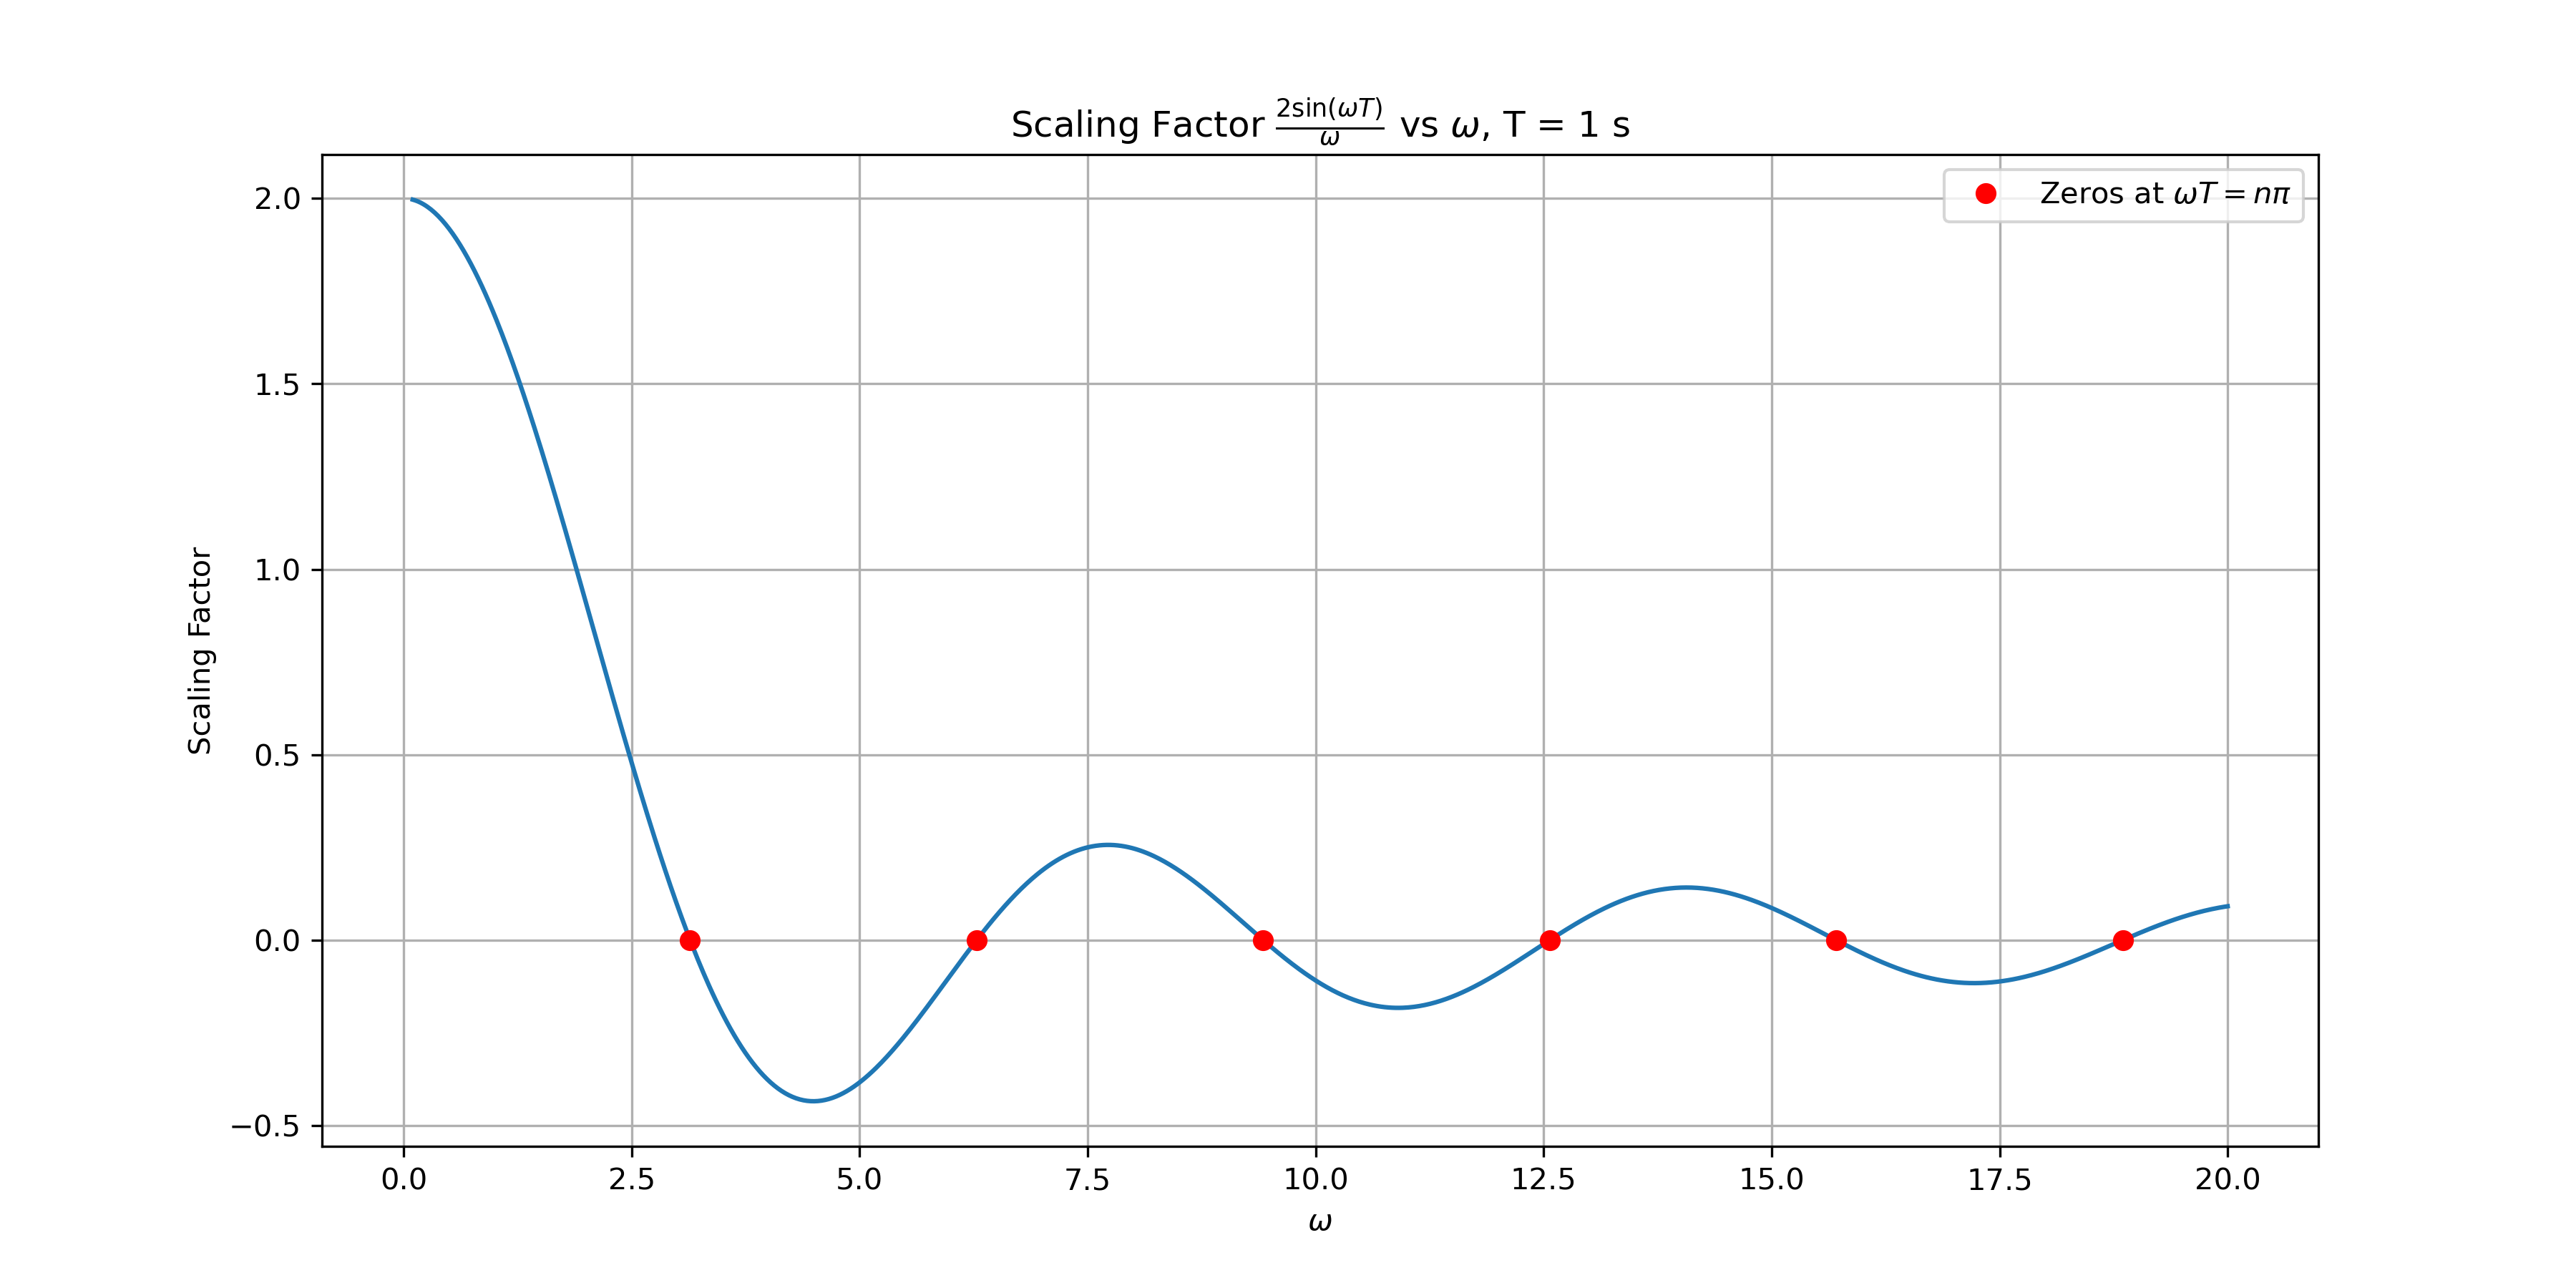
\includegraphics[width=0.95\textwidth]{codes/codes_sin_3_and_smoothening/figs/scaling_factor_analysis.png}
    \end{center}
    \caption{Amplitude/Scaling factor dependence on $\omega$ taking $T = 1s$}
\end{figure}
\FloatBarrier

The amplitude ratio is sinusoidal with respect to T with angular frequency $\omega$ when all the other parameters are constant.

\begin{figure}[!ht]
    \begin{center}
        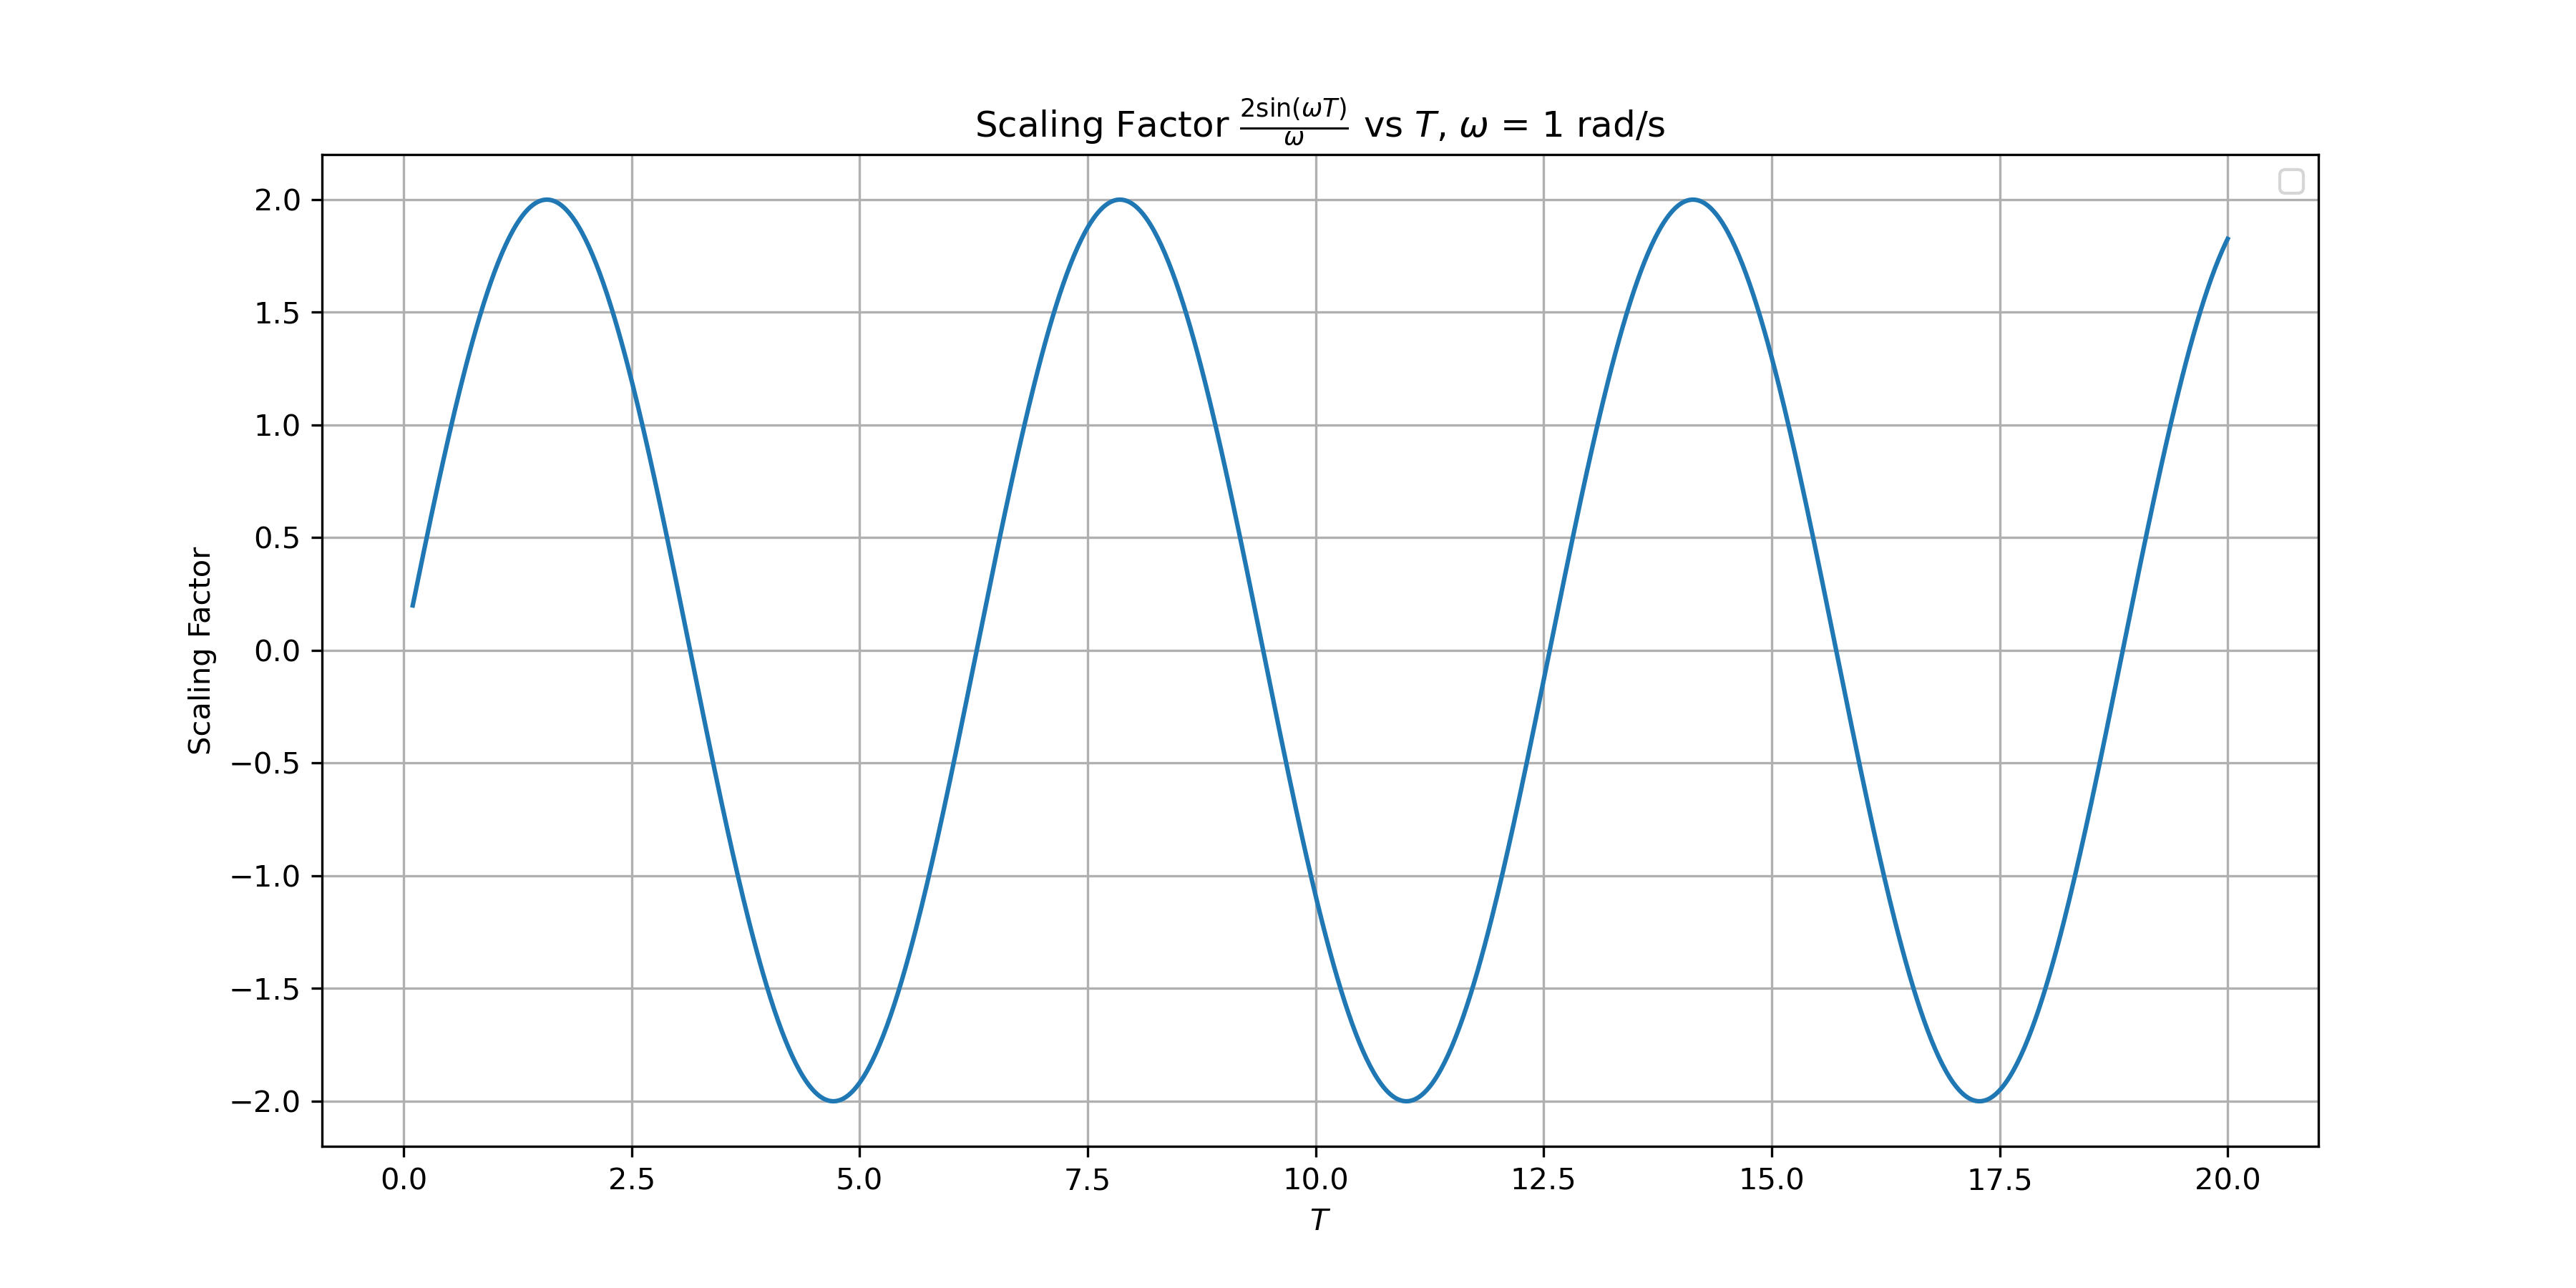
\includegraphics[width=0.95\textwidth]{codes/codes_sin_3_and_smoothening/figs/scaling_factor_analysis_T.png}
    \end{center}
    \caption{Amplitude/Scaling factor dependence on $T$ taking $w = 1 rad/s$}
\end{figure}
\FloatBarrier

\subsection{More analysis on Effect of Kernel Width (T)}
The convolved ouput's amplitude ratio is sinusoidal with respect to T when all the other parameters are constant.

\begin{figure}[!ht]
    \begin{center}
        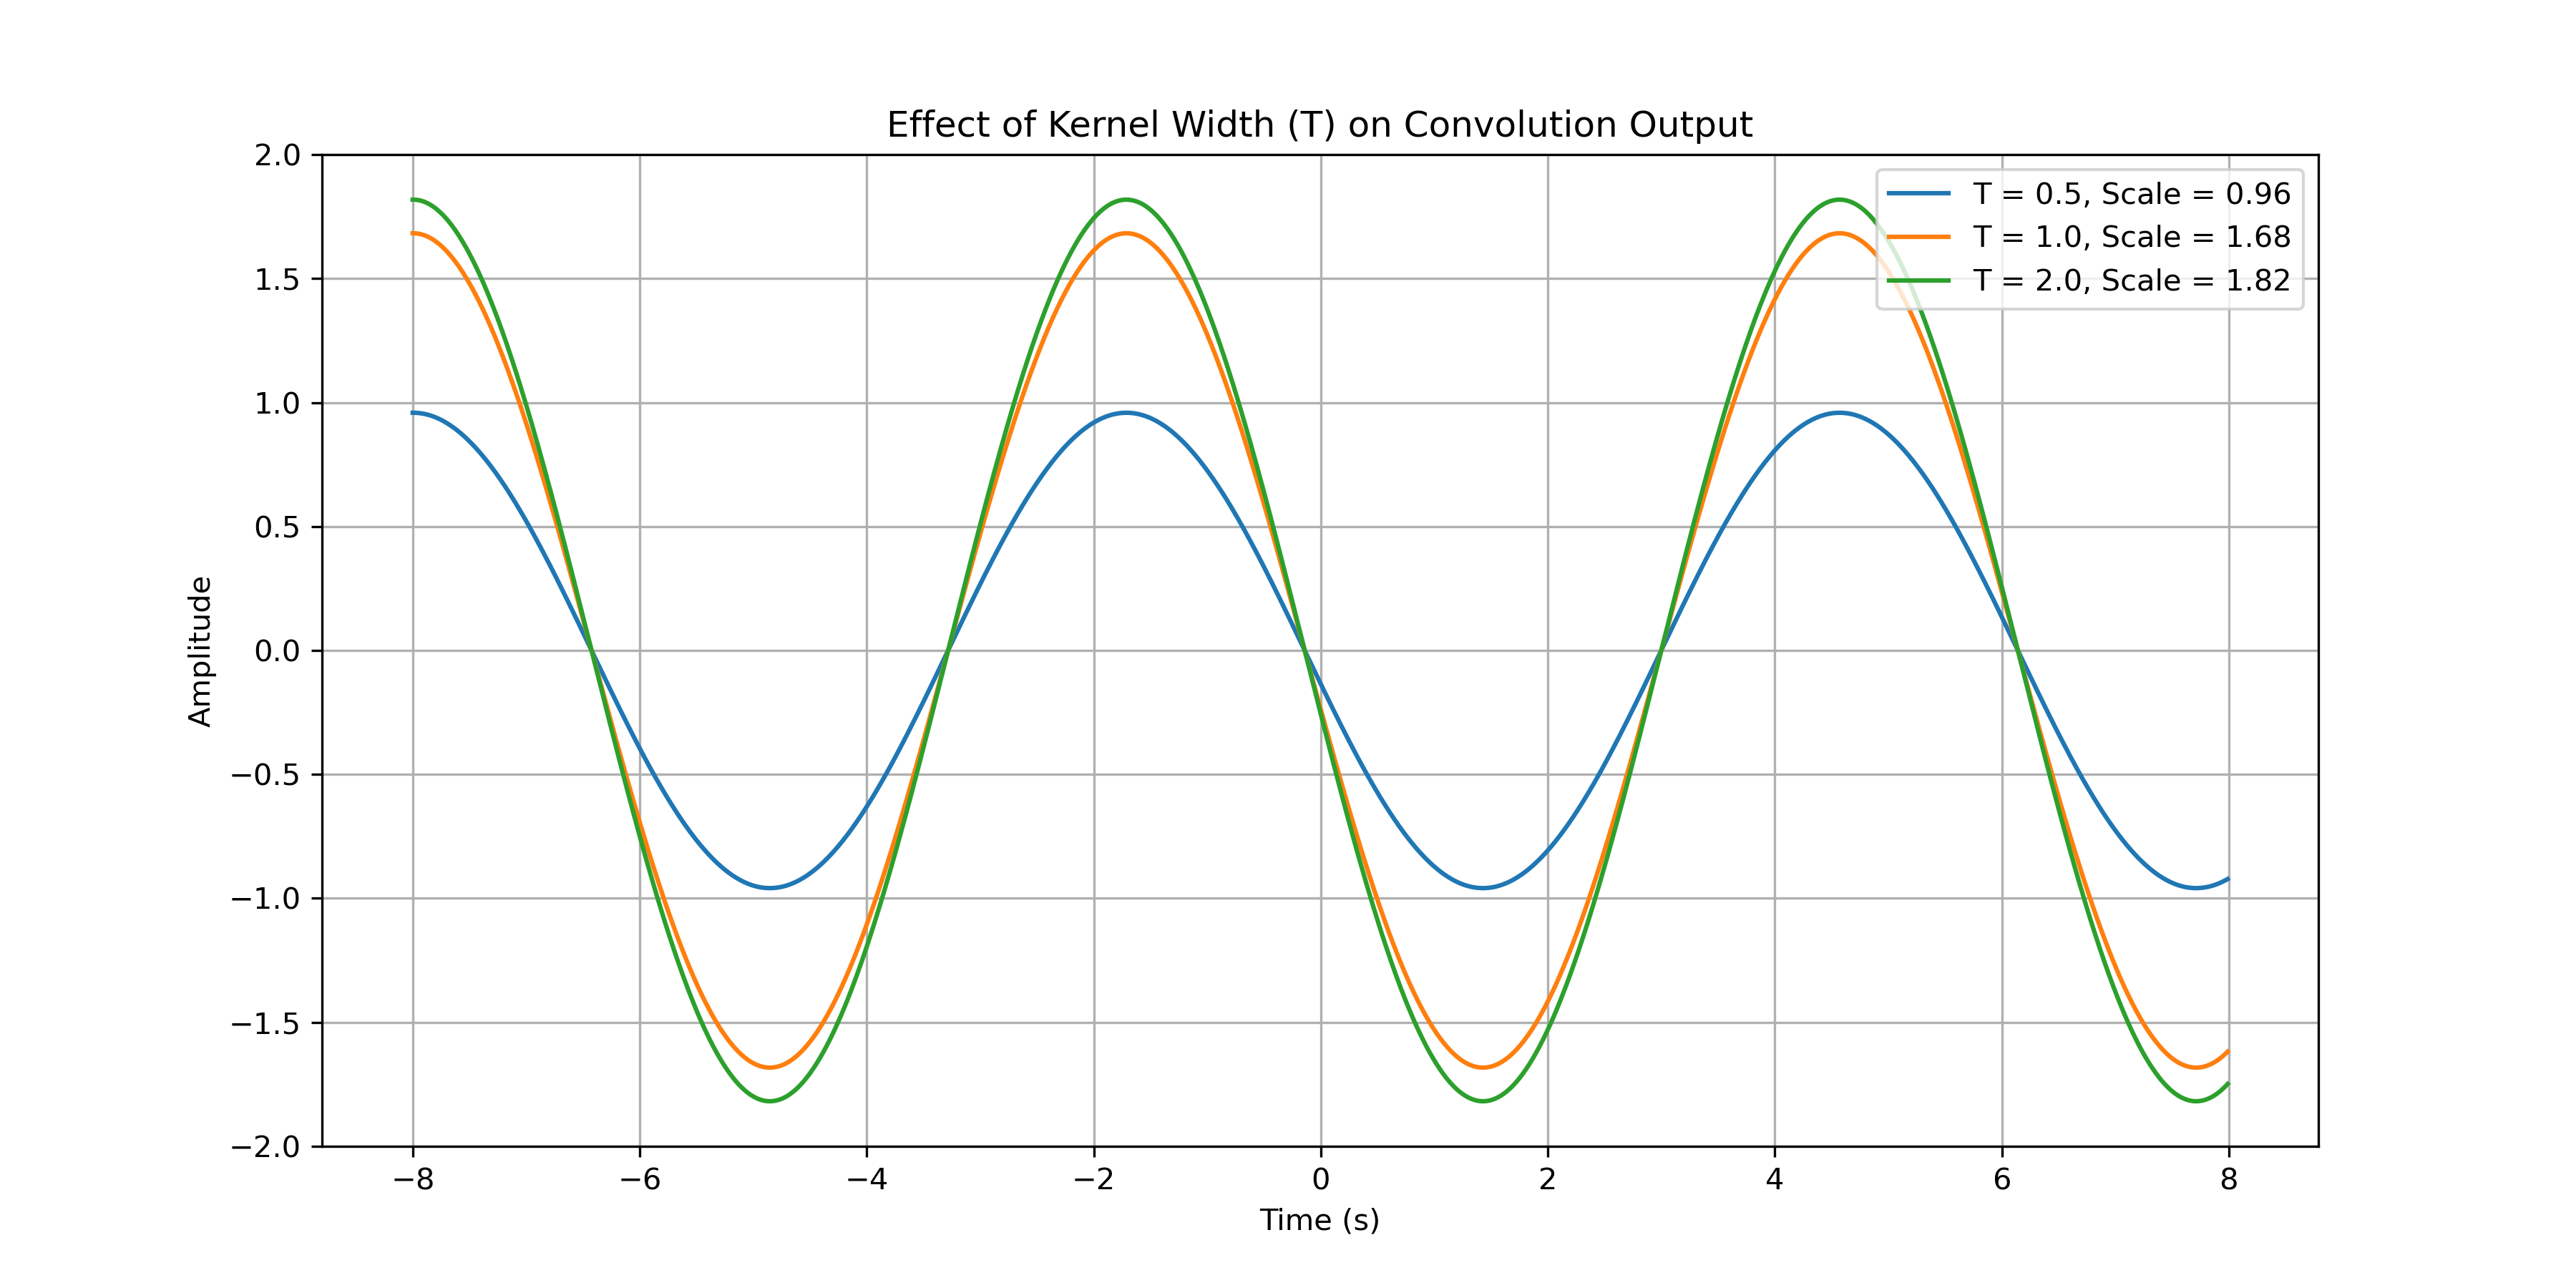
\includegraphics[width=0.95\textwidth]{codes/codes_sin_3_and_smoothening/figs/varying_T_effect.png}
    \end{center}
    \caption{Effect of Varying T on the Convolved output}
\end{figure}
\FloatBarrier
